\begin{figure}[H]
\centering

\begin{subfigure}{.33\textwidth}
  \centering
  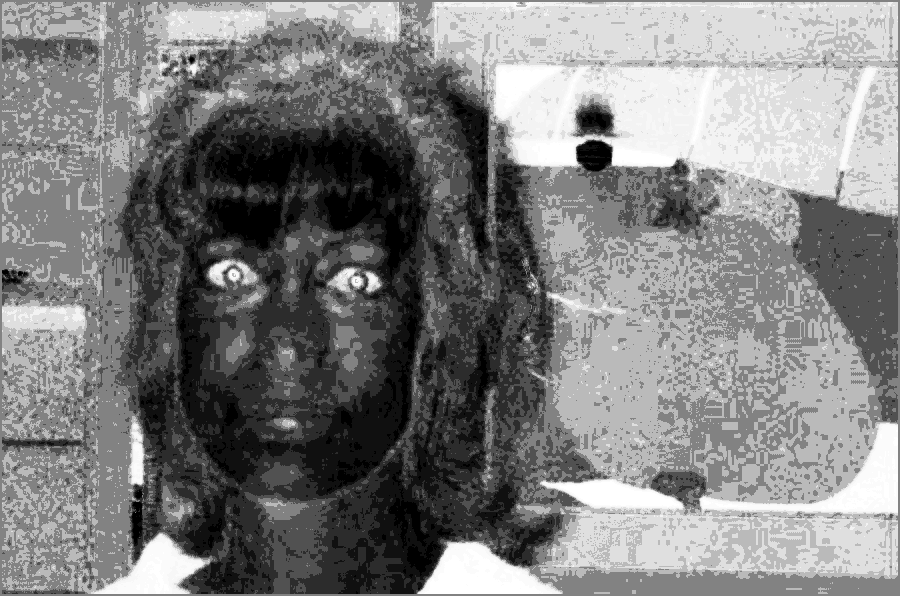
\includegraphics[width=0.95\textwidth]{img/fd2/EyeMapChroma.png}
  \caption{}
  % \label{fig:sub1}
\end{subfigure}%
\begin{subfigure}{.33\textwidth}
  \centering
  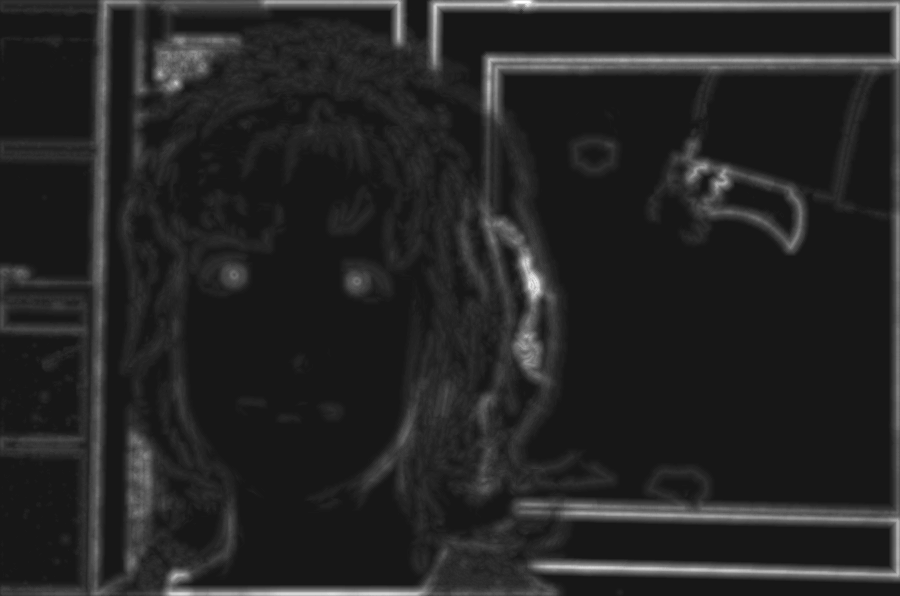
\includegraphics[width=0.95\textwidth]{img/fd2/EyeMapLuma.png}
  \caption{}
  % \label{fig:sub1}
\end{subfigure}%
\begin{subfigure}{.33\textwidth}
  \centering
  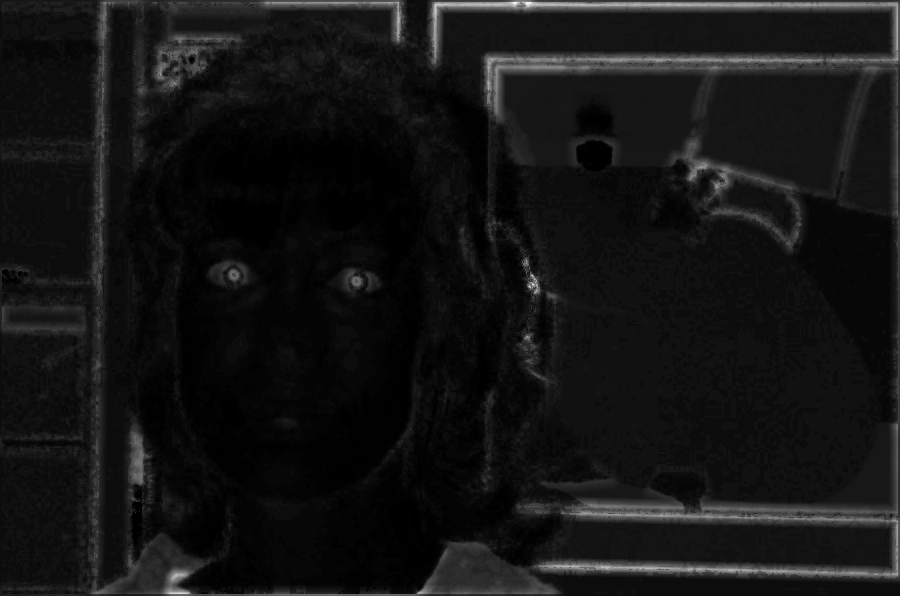
\includegraphics[width=0.95\textwidth]{img/fd/OriginalEyeMap.png}
  \caption{}
  % \label{fig:sub1}
\end{subfigure}%

\begin{subfigure}{.33\textwidth}
  \centering
  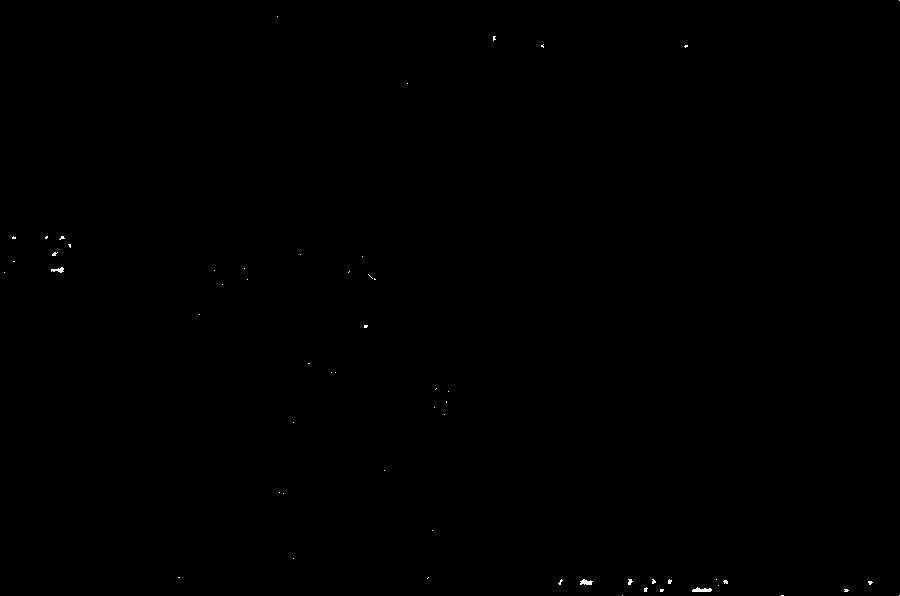
\includegraphics[width=0.95\textwidth]{img/fd/OverSaturatedMask.png}
  \caption{}
  % \label{fig:sub1}
\end{subfigure}%
\begin{subfigure}{.33\textwidth}
  \centering
  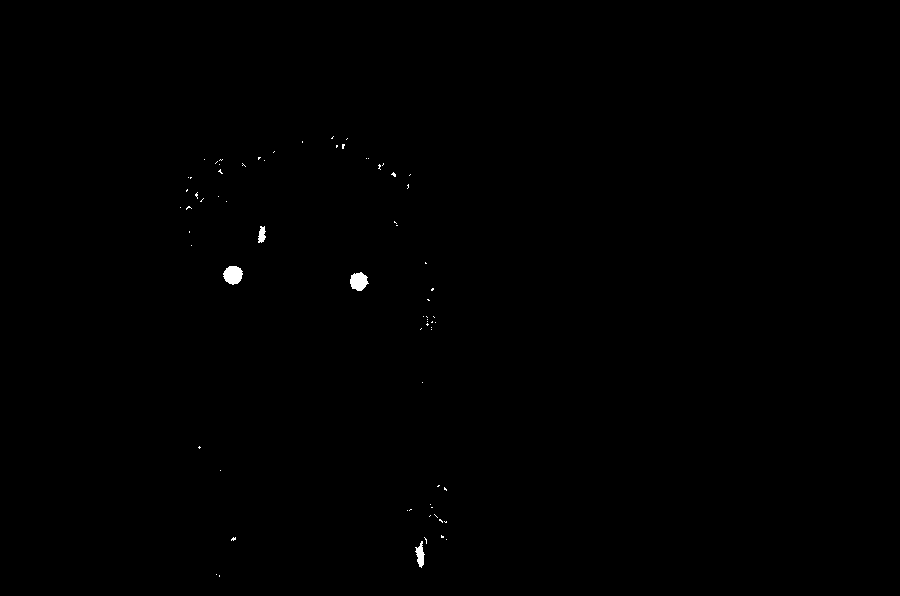
\includegraphics[width=0.95\textwidth]{img/fd/FilteredFaceMaskEyesReal.png}
  \caption{}
  % \label{fig:sub1}
\end{subfigure}%
\begin{subfigure}{.33\textwidth}
  \centering
  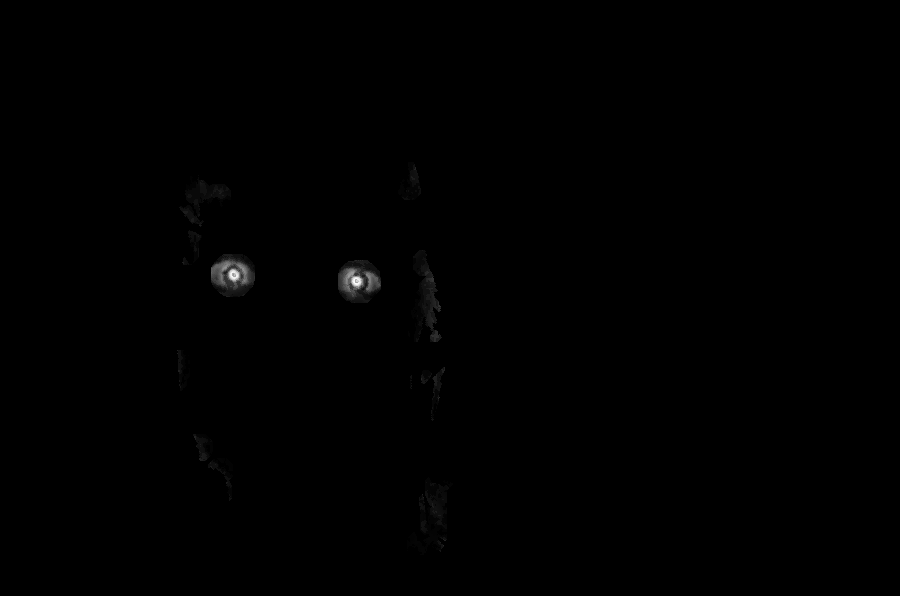
\includegraphics[width=0.95\textwidth]{img/fd/EyeMap2.png}
  \caption{}
  % \label{fig:sub1}
\end{subfigure}%

\caption{Process of computing the eyes' locations.}
\label{fig:eyeMap}
\end{figure}